\documentclass{jsarticle}
\usepackage[dvipdfmx,hiresbb]{graphicx}

\begin{document}

\title{音楽再生と時間の関係}
\author{藤賀雄太}
\date{2012年12月1日}
\maketitle

\section{イントロダクション}
\subsection{あらまし}
iPodなどのモバイルプレイヤーの登場により音楽視聴はいつでも可能なものになった。
本研究では時刻によって、音楽の聴き方がどのように変化するのかを調べた。
この研究が音楽の自動選曲システムの向上に貢献できればと考える。
研究の結果、時間情報はfoobarでした。

\subsection{キーワード}
iTunes, iPod, 時間情報, レコメンドサービス, ライフログ

\section{分析手順}
\begin{enumerate}
\item
被験者10名(iTunesをいつも利用して音楽を聴いている大学生)から履歴ファイル(xmlファイル)をメール添付でもらう。

\item
被験者に自分の生活を曜日毎にアンケートシートに書いてもらう。
\begin{center}
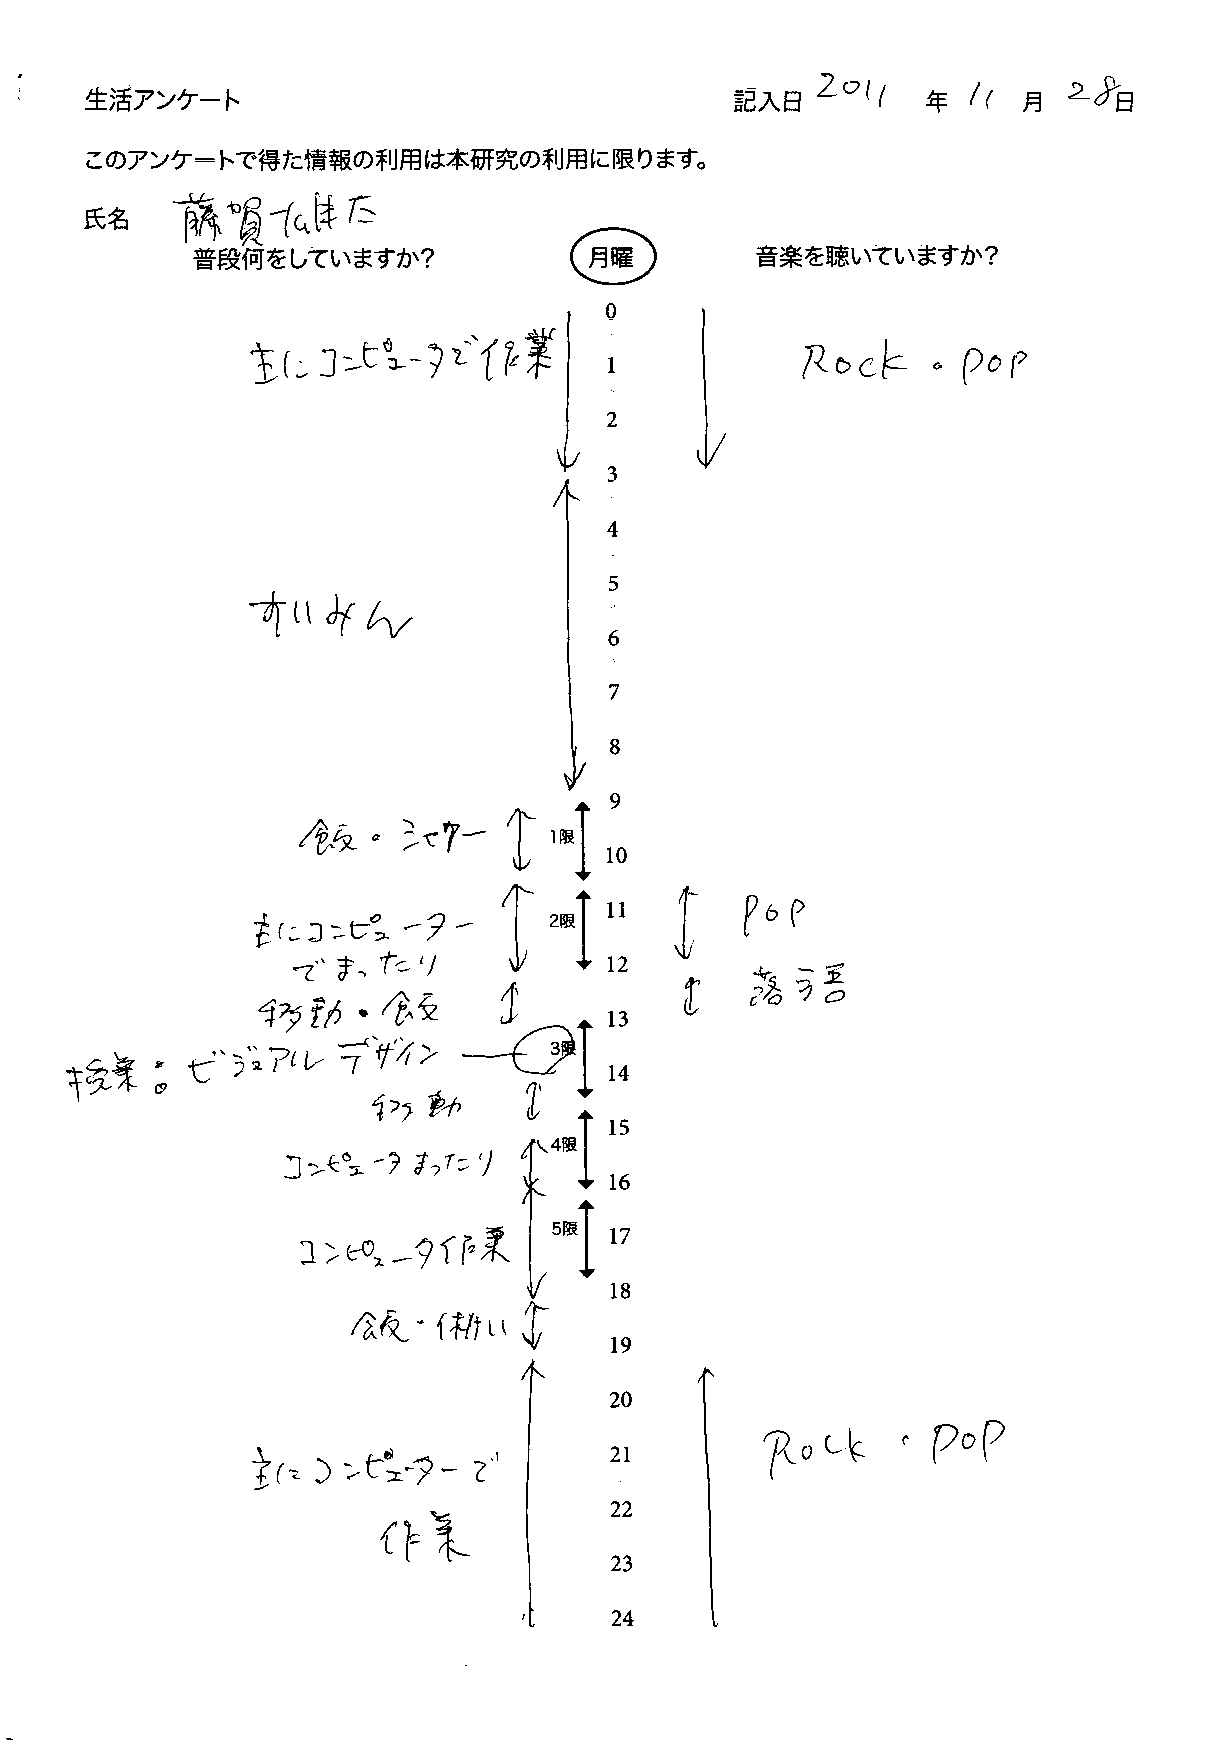
\includegraphics[width=7cm]{musicLifeSheet_sample.pdf}
\end{center}

被験者に渡したのは、0時から24時までを30分刻みで目盛りを付けたもので、普段の生活と、普段の音楽聴取を記入してもらうもので、月曜日から日曜日までの合計7枚のものである。
不規則な生活、気まぐれな音楽再生など、毎週規則正しく定期的に書けない部分も備考として記入してもらう。
なお、iTunesをシャッフルで聴いたかどうかは、iTunesに記録されていないため、備考に書いてもらう。
\item
pythonを用いて、履歴ファイルから、以下の情報だけを読み取って、テキストファイルに書き出す。
\begin{itemize}
\item
楽曲のジャンル
\item
最後に聴いた日付・時間
\item
再生回数
\end{itemize}

\item
Rを用いて、2でつくったテキストファイルを読み込んで、一度以上再生された楽曲について、曜日毎に分類し、さらに、0時から24時まで1時間刻みのヒストグラムをつくる。そして、ヒストグラムのデータをcsvファイルとして保存する。なお、ヒストグラムを画像ファイル(pngデータ)として書き出す。

\item
openFrameworksを用いて、csvファイルから、0時から24時まで30分刻みのヒストグラムを月曜から日曜までの累積棒グラフの形式でつくる。棒グラフの棒の数は、24(1時間刻み)*7(月曜から日曜)=168本になる。総合再生回数がベスト5のものだけをカラーにして、それ以外をその他としてグレーで描画した。

\begin{center}
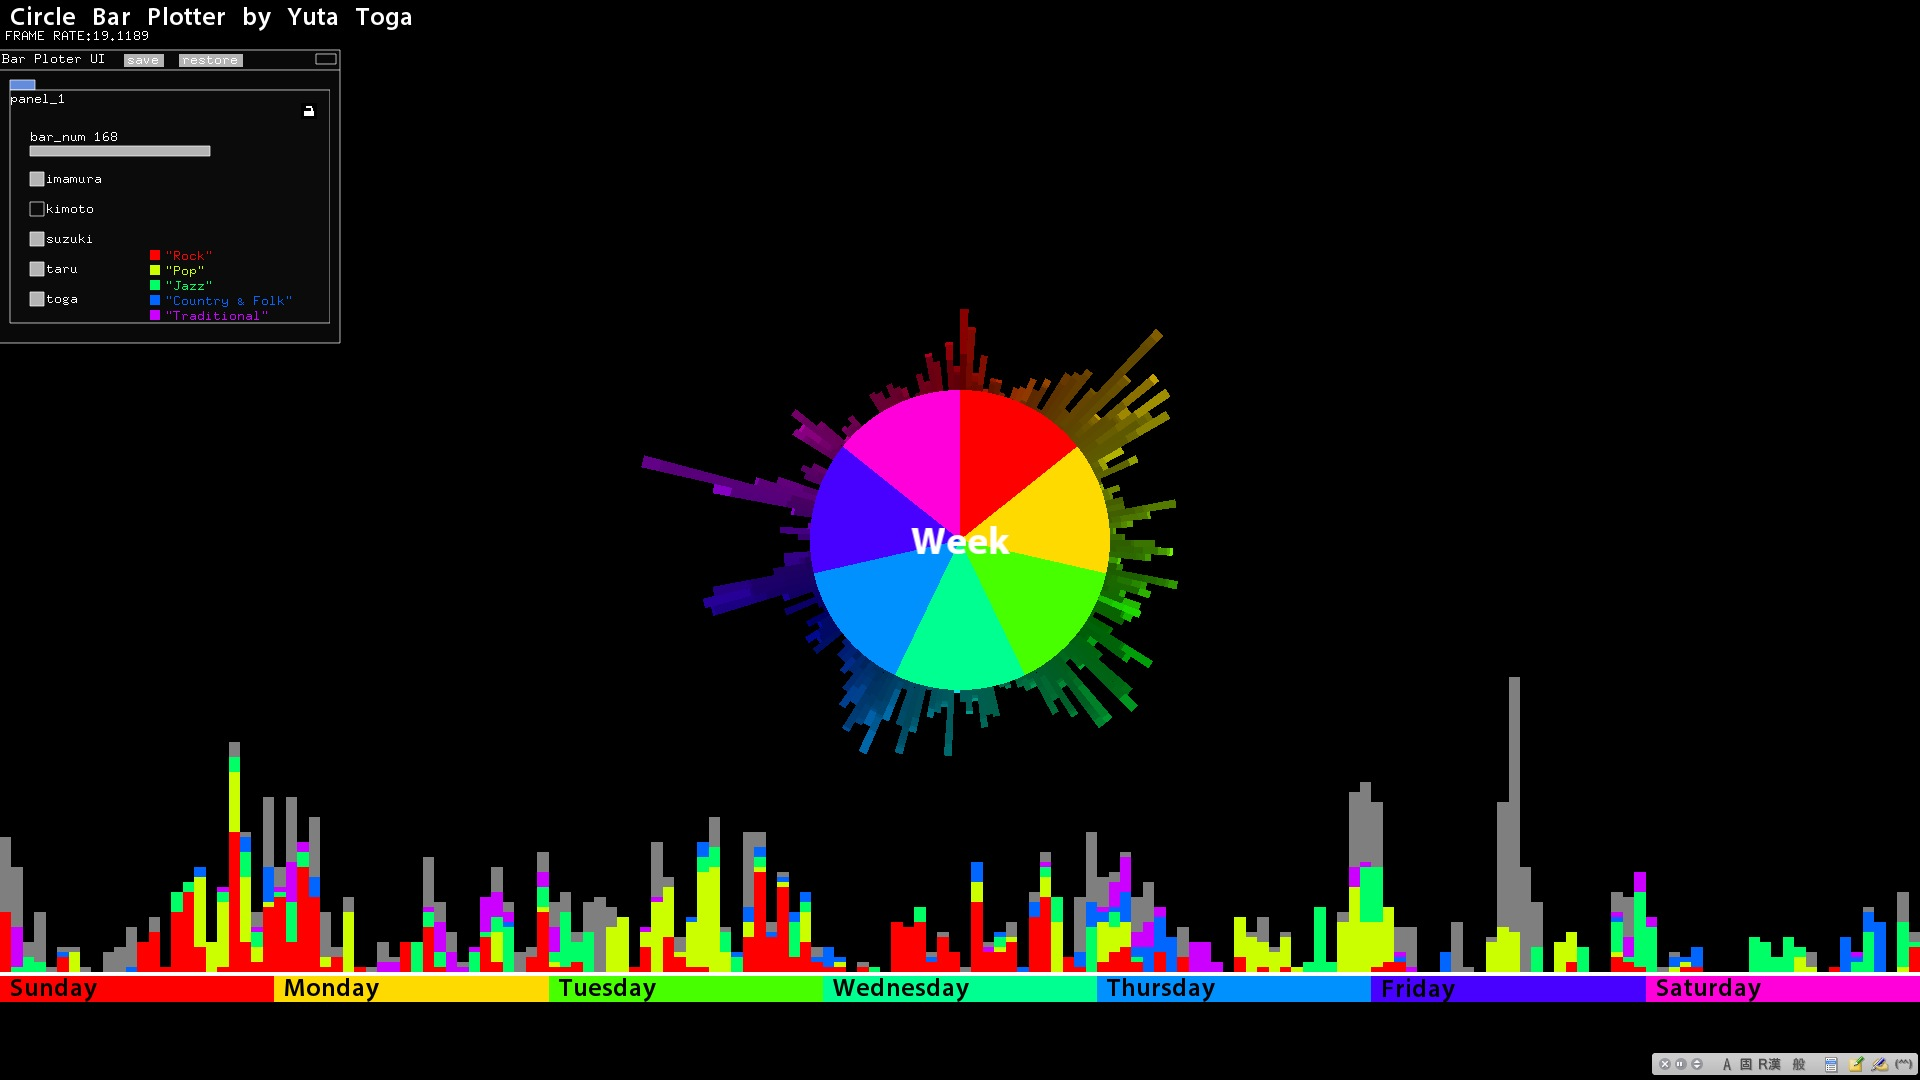
\includegraphics[width=14cm]{graph_sample.jpg}
\end{center}

\item
ヒストグラムの見た目から、聴いている音楽と、時間に相関があるかを調べる。

\item
被験者のアンケートシートで得た情報と、xmlファイルから読み取ったものとの比較を行う。

\item
質問があったらインタビューを行う。

\end{enumerate}

\section{結果}
ヒストグラムはこうなりました。寝ている時間が推測できる。必ず聴いていない時間が存在することがあり、その時間は定期的な会議などがあることが多かった。金曜の夜だけ多く聴いているというような、曜日による偏りが見られた。

\section{分析}
iTunesの仕様により、再生履歴は最後に聞いた時間の情報しか残っていない。すなわち、10回聞いたの楽曲がある場合も、いつ聞いたのかという情報は最後の10回目しか記録されておらず、1回目から9回目の情報は上書きによって失われている。そのため、今回の研究では、アンケートにおいて、シャッフルで再生しているかどうかを聞き出すことにした。
 もし、月曜日に特に音楽を聞いているという場合、なぜ月曜にそうなるのかという理由は聴いてみないとわからないため、アンケートで得られた、普段の生活を参照した。
また、この時間あなたは授業などで音楽を聴けない状況ではないですか?というようにインタビューによって利用者の音楽試聴状況を推測することができた。これは、今後、自動選曲システムにおいて、設定をすべてユーザーに任せるのではなく、もしかして、金曜の夜はあまりロックは聴かないですね?というような、質問形式で数問回答させることにより、ユーザーの音楽試聴状況に沿った選曲ができる(沿うことがよいリコメンドかどうかは別として)可能性を示唆する。
ランダムに再生している人と、時間と音楽再生に偏り(相関がある)人にどう分かれるのかを調べる。

\section{考察}
アンケートに書かれていることと、xmlファイルから得られた音楽再生の状況が異なる場合、一致する場合それぞれについて、なぜそうなるのかを考察する。
生活のコンテキスト、特に時間情報が音楽再生に影響力をもっているかどうかを考察し、音楽リコメンドサービスについての発展を考える。

\section{備考}
研究資料および、プログラムの一部は、(個人情報は含まない)
yutatoga.com/thesisからダウンロードできる。


\end{document}